%%%%%%%%%%%%%%%%%%%%%%%%%%%%%%%%%%%%%%%%%%%%%%%%%%%%%%%%%%%%%%%%%%%%%%%%
\section{Kombinatorik (Zählen)}
\subsection{Produktregel: Die Für–jedes–gibt–es–Regel (FJGE)}
Fur jede der $n_1$ Möglichkeiten gibt es eine von der
ersten Position unabhängige Anzahl $n_2$ Möglichkeiten für den Rest.
\[ = n_1 \cdot n_2 \text{ Möglichkeiten } \]

\subsection{Permutationen: Reihenfolge}
Anzahl Anordnungen: Auf wieviele Arten kann man $n$ Objekte anordnen?
\[ = n! \text{ Arten} \]

\subsection{Kombinationen: Auswahl}
Auf wieviele Arten kann man $k$ Objekte aus $n$ auswählen?
\[ = C^n_k=\binom{n}{k} = \frac{n!}{k!(n-k)!} \text{ Arten} \]
Dieser "`Binomialkoeffizient"' lässt sich auf dem Taschenrechner
TI-36XII mit \texttt{n nCr k} (unter \texttt{PRB}), mit dem Voyage 200
mit \texttt{nCr(n,k)}, in Sage mit \texttt{binomial(n,k)} und in 
Octave/Matlab mit \texttt{nchoosek(n,k)} berechnen.

Auf wieviele Arten kann man $k$ Mal eine Auswahl aus $n$ Objekten
treffen?
\[ = n^k \text{ Arten} \]

\subsection{Hypergeometrische Verteilung}

Die Wahrscheinlichkeit, bei einer $n$ Elemente umfassenden Stichprobe
aus einer $N$ Elemente grossen Gesamtheit, in der $M$ ein bestimmtes
Merkmal tragen, deren $m$ mit dem Merkmal zu finden ist:
\[ = \frac{\begin{pmatrix}M\\n\end{pmatrix} \cdot
  \begin{pmatrix}N-M\\n-m\end{pmatrix}}
  {\begin{pmatrix}N\\n\end{pmatrix}} \]

Wie gross ist die Wahrscheinlichkeit $i$ Items einer Art (von welcher es
$a$ gibt) aus der Menge (mit Grösse $m$) mit einer Stichprobengrösse $s$
auszuwählen?
\[ = \frac{\begin{pmatrix}m-a\\s-i\end{pmatrix} \cdot
  \begin{pmatrix}a\\i\end{pmatrix}}
  {\begin{pmatrix}m\\s\end{pmatrix}} \]

%%%%%%%%%%%%%%%%%%%%%%%%%%%%%%%%%%%%%%%%%%%%%%%%%%%%%%%%%%%%%%%%%%%%%%%%
\section{Ereignisse und Wahrscheinlichkeit}
\subsection{Wahrscheinlichkeitsexperimente}
\begin{itemize}
  \item Alle möglichen Versuchsausgänge $\Omega$
  \item Elementarereignis $\omega \in \Omega$
  \item Ereignis $A \subset \Omega$
  \item Verschiedene Elementarereignisse $\omega \in A$
  \item Ereignis $A$ tritt ein $\Leftrightarrow \omega \in A$
  \item Wahrscheinlichkeit dass Ereignis $A$ eintritt ist $P(A)$
\end{itemize}

\subsection{Eigenschaften von Wahrscheinlichkeiten}
\begin{itemize}
  \item Laplace-Ereignisse: Alle Elementarereignisse haben die gleiche
    Wahrscheinlichkeit
  \item $P(A) = \frac{|A|}{|\Omega|}$: Wahrscheinlichkeit von
    Elementarereignis $A$
  \item $0 \le P(A) \le 1$: Wahrscheinlichkeit ist immer zwischen $0$
    und $1$
  \item $P(A) < P(B)$: Die Wahrscheinlichkeit für das Ereignis $A$ ist
    kleiner als für $B$
  \item $P(\Omega) = 1$: Das sichere Ereignis tritt immer ein
  \item $P(\emptyset) = 0$: Das unmöglich Ereignis tritt nie ein
\end{itemize}

\subsection{Rechnen mit Wahrscheinlichkeiten}
\begin{itemize}
  \item $P(A \cap B)$: Ereignis $A$ und Ereignis $B$ tritt ein
    \begin{itemize}
      \item Falls unabhängig: $= P(A) \cdot P(B)$
      \item Drei Ereignisse:
        $P(A \cap B \cap C) = P(A) \cdot P(B) \cdot P(B)$
      \item Falls abhängig: Nicht alleine aus $P(A)$ und $P(B)$
        berechenbar!
    \end{itemize}
  \item $P(A \cup B) = P(A) + P(B) - P(A \cap B)$\footnote{Ein-
    Ausschaltformel}: Ereignis $A$ oder Ereignis $B$ tritt ein
    \begin{itemize}
      \item Falls sich $A$ und $B$ nicht überschneiden\footnote{
        Paarweise disjunkt: $A$ und $B$ treffen nicht gleichzeitig ein}:
        $= P(A) + P(B)$
      \item Drei Ereignisse: $P(A \cup B \cup C) \\ = P(A) + P(B) + P(C)
        - P(A \cap B) - P(A \cap C) - P(B \cap C) + P(A \cap B \cap C)$
    \end{itemize}
  \item $P(A \setminus B) = P(A) - P(A \cap B)$: Ereignis $A$ tritt ein, aber ohne
    Ereignis $B$
  \item $P(\bar{A}) = P(\Omega \setminus A) = 1 - P(A)$: Ereignis $A$
    tritt nicht ein
  \begin{itemize}
    \item Bedingte Wahrscheinlichkeit: $P(\bar{A}|B) = 1 - P(A|B)$
  \end{itemize}
\end{itemize}

\subsection{Bedingte Wahrscheinlichkeit}
Wahrscheinlichkeit, dass $A$ eintritt, wenn wir schon wissen, dass $B$
eingetreten ist.\footnote{Somit gilt auch: $P(A) = P(A|\Omega)$}
\[ P(A|B) = \frac{P(A \cap B)}{P(B)} \]
Falls $A$ und $B$ unabhängig sind (z.~B. Behauptung eines Kritikers):
\[ P(A|B) = \frac{P(A) P(B)}{P(B)} = P(A) \]
und
\[P(A) = P(A|B) = P(A|\overline{B}) \text{ und } P(B) = P(B|A)
= P(B|\overline{A})\]


\subsection{Satz der totalen Wahrscheinlichkeit}
Aus Einzelfällen kann man die Gesamtsituation zusammenstellen:
\[ P(A) = \sum_{i=1}^{n}P(A|B_i) \cdot P(B_i) \]

\subsection{Satz von Bayes}
Mit dem Satz von Bayes kann man die Schlussrichtung umkehren
\footnote{Weil $P(A|B) \cdot P(B) = P(A \cap B) = P(B|A) \cdot P(A)$}:
\[ P(A|B) = P(B|A) \cdot \frac{P(A)}{P(B)} \]

%%%%%%%%%%%%%%%%%%%%%%%%%%%%%%%%%%%%%%%%%%%%%%%%%%%%%%%%%%%%%%%%%%%%%%%%
\section{Erwartungswert und Varianz}
\subsection{Erwartungswert}
\subsubsection{Begriffe}
\begin{itemize}
  \item Zufallsvariable $X$ ordnet Elementarereignissen $\omega$ Werte
    zu: $X: \Omega \rightarrow \mathbb{R}$
  \item Erwartungswert (Zufallsvariable im Mittel): \\
    $E(X) = \sum_{Werte} \text{Wert } \cdot
    \text{Wahrscheinlichkeit } = \sum_i w_i \cdot P(w_i)$
  \item Empirischer Erwartungswert = arithmetisches Mittel:
    $E(X) = \frac{1}{n} \sum_{i=1}^n x_i$
\end{itemize}
\subsubsection{Spezielle Zufallsvariable}
Charakteristische Funktion von $A$:
\[ \chi_A = \begin{cases}1 & w \in A \\ 0 & sonst \end{cases} \]
\[ E(X) = 0 \cdot P(\bar{A}) + 1 \cdot P(A) = P(A) \]

\subsubsection{Rechnen mit Erwartungswerten}
\begin{itemize}
  \item Multiplikation mit einem Faktor: $E(\lambda X) = \lambda E(X)$
  \item Addition zweier Zufallswerte: $E(X + Y) = E(X) + E(Y)$
  \item Produkt zweier Zufallswerte: $E(X \cdot Y) \ne E(X) \cdot E(Y)$
  \begin{itemize}
    \item Potenzieren (immer abhängig): $E(X^2) \ne E(X)^2$
    \item Wenn die zwei Werte sich nicht beeinflussen
      (unabhängig): $E(X \cdot Y) = E(X) \cdot E(Y)$
  \end{itemize}
  \item Erwartungswert einer Konstante $c$: $E(c) = c$
\end{itemize}

\subsection{Varianz (Streubreite)}
\subsubsection{Begriffe}
\begin{itemize}
  \item Varianz (Mass für die mittlere Abweichung):
    $\operatorname{var}(x) = E((X - E(X))^2) = E(X^2) - E(X)^2 =
    \sum((x-E(x))^2 \cdot p(x))$
  \item Je grösser die Varianz, desto Wahrscheinlicher sind grosse
    Abweichungen vom Mittelwert.
  \item Kovarianz (Verschiebungssatz):
    $\operatorname{cov}(X,Y) = E(XY) - E(X)E(Y)$
  \item Standardabweichung: Abstand ($\pm$) zum Erwartungswert:
    $\sigma = \sqrt{\operatorname{var}(x)}$
\end{itemize}
\subsubsection{Rechenregeln für Varianz}
\begin{itemize}
  \item Multiplikation mit einem Faktor:
    $\operatorname{var}(\lambda X) = \lambda^2 \operatorname{var}(X)$
  \item Addition (nur wenn $X$ und $Y$ unabhängig):
    $\operatorname{var}(X+Y) = \operatorname{var}(X) + \operatorname{var}(Y)$
    \begin{itemize}
      \item Achtung: ($(-x)^2 = +x$): $\operatorname{var}(X-Y) =
      \operatorname{var}(X) + \operatorname{var}(-Y) =
      \operatorname{var}(X) + \operatorname{var}(Y)$
    \end{itemize}
  \item Multiplikation: $\operatorname{var}(X \cdot Y) = \operatorname{var}(X)
    \operatorname{var}(Y) + \operatorname{var}(Y)E(X)^2 + \operatorname{var}(X)E(Y)^2$
  \item Varianz einer Konstante $c$: $\operatorname{var}(c) = 0$
  \item Kovarianz als Verallgemeinerung der Varianz:
    $\operatorname{var}(X) = \operatorname{cov}(X,X)$
\end{itemize}

\subsection{Mittelwert}
\subsubsection{Begriffe}
\begin{itemize}
  \item Erwartungswert der Zufallsvariablen $X$: $\mu = E(X)$
  \item Varianz: Abweichung der Zufallsvariabeln von ihrem
    Erwartungswert: $X -\mu$
  \item Wie häufig überschreitet die Abweichung $\varepsilon$?
  \item Wie wahrscheinlich ist es, dass die Abweichung gross ist?
    $P(|X - \mu| > \varepsilon)$
  \item Faustregel: 10 mal mehr Genauigkeit = 100 mal mehr Arbeit.
\end{itemize}
\subsubsection{Ungleichung von Tschebyscheff}
Genauigkeit des Mittelwertes: Wahrscheinlichkeit, dass Zufallsvariable
$X$ um mehr als $\varepsilon$ vom Erwartungswert abweicht:
\[P(|X-\mu| > \varepsilon) \le \frac{\operatorname{var}(X)}{\varepsilon^2} \]
\subsubsection{Wie gut ist der Mittelwert?}
\begin{itemize}
  \item Mittelwert: $M_n = \frac{X_1 + X_2 + \ldots + X_n}{n}$
  \item Erwartungswert: $E(X_i) = E\left( \frac{X_1 + X_2 + \ldots +
  X_n}{n}\right) =  \frac{E(X_1) + E(X_2) + \ldots + E(X_n)}{n} = \mu$
  \item Varianz: $\operatorname{var}(X_i) = \sigma^2$
  \item Varianz: $\operatorname{var}(M_n) = \frac{1}{n^2} \sum_{i=1}^n
  \operatorname{var}(X_i) = \frac{\sigma^2}{n}$
\end{itemize}
\paragraph{Bernoullis Gesetz der grossen Zahlen}
Die Wahrscheinlichkeit, dass der Mittelwert von $n$ unabhängigen
Zufallsvariabeln mit Mittelwert $\mu$ und Varianz $\sigma^2$ mehr als
$\varepsilon$ von $\mu$ abweicht, ist:
\[P(|X-\mu| > \varepsilon) \le \frac{\operatorname{var}(X)}{\varepsilon^2} \]
Die Abweichung ist unwahrscheinlich, wenn:
\begin{itemize}
  \item Varianz ist klein (genaues Messgerät)
  \item $\varepsilon$ ist gross (man ist toleranter)
  \item $n$ ist gross (viele Messungen)
\end{itemize}

\subsection{Lineare Regression}
Seien $X$ und $Y$ zwei reelle Zufallsvariablen. Die Gerade mit der
Gleichung $y = ax + b$ minimiert die Varianz $\operatorname{var}(aX + b -Y)$
genau dann, wenn
\begin{align*}
  a & = \frac{\operatorname{cov}(X,Y)}{\operatorname{var}(X)} = \frac{E(XY)
        - E(X)E(Y)}{E(X^2) - E(X)^2} \\
  b & = E(Y) - E(X)a
\end{align*}
Die Regression ist umso genauer, je näher der Regressionskoeffizient $r$
bei $\pm 1$ liegt. Zudem hat $r$ immer das gleiche Vorzeichen wie die
Steigung der Regressionsgerade.
\[ r = \frac{\operatorname{cov}(X,Y)}
  {\sqrt{\operatorname{var}(X)\operatorname{var}(Y)}} \]

\begin{itemize}
  \item Ist $r = 0$: Kein linearer Zusammenhang zwischen $x$ und $y$
    (Unabhängig)
  \item Ist $r = 1$: Kein Fehler bei der Approximation
\end{itemize}

Zur Berechnung der Regression eignet sich folgende Tabelle sehr gut,
damit man alle Werte im Überblick hat:

\begin{tabular}{|l|l|l|l|l|l|}
  \hline
  $i$    & $x_i$    & $y_i$    & ${x_i}^2$    & ${y_i}^2$  & $x_i \cdot y_i$ \\
  \hline
  \hline
  1      & $x_1$    & $y_1$    & ${x_1}^2$    & ${y_1}^2$  & $x_i \cdot y_i$ \\
  \vdots & \vdots   & \vdots   & \vdots       & \vdots     & \vdots \\
  \hline
  \hline
  $E$ & $E(x_i)$ & $E(y_i)$ & $E({x_i}^2)$ & $E({y_i}^2)$ & $E(x_i \cdot y_i)$ \\
  \hline
\end{tabular}
\begin{itemize}
  \item Punkt auf X-Achse: $x_i$
  \item Punkt auf Y-Achse: $y_i$
  \item $E(X)$ ist das arithmetische Mittel
\end{itemize}

%%%%%%%%%%%%%%%%%%%%%%%%%%%%%%%%%%%%%%%%%%%%%%%%%%%%%%%%%%%%%%%%%%%%%%%%
\section{Wahrscheinlichkeitsverteilung}
\subsection{Begriffe}
\begin{itemize}
  \item Verteilungsfunktion: $F(x) = P(X \le x)$
  \item Die Verteilungsfunktion $F$ einer Zufallsvariablen $X$, $F(x) =
    P(X \leq x)$, zeigt die Wahrscheinlichkeit dafür, dass $X$ den Wert
    $x$ nicht überschreitet.
  \item Monoton wachsend: $F(b) - F(a) = P(a < X \leq b) \geq 0$ falls
    $a \leq b$
  \item Ableitung von $F$ (Wahrscheinlichkeitsdichte / Dichtefunktion):
    $F'(x) = \varphi(x)$
  \begin{itemize}
    \item[$\Leftrightarrow$] $F(x) = \int_{-\infty}^{x} \varphi(\tau) d\tau$
    % TODO Verify
  \end{itemize}
  \item Formen der Zufallsvariabeln
  \begin{itemize}
    \item Diskret: Zufallsvariable kann endlich viele Werte annehmen.
      ($F$ ist stückweise konstant (Treppenstufen))
    \item Stetig: Zufallsvariable kann unendlich viele Werte annehmen.
      ($F$ ist ist stetig)
  \end{itemize}
\end{itemize}

\subsection{Eigenschaften der Verteilungsfunktion}
\begin{itemize}
  \item Verteilfunktion zwischen $0$ und $1$: $0 \le F(x) \le 1$
  \item Grenzwerte: $\lim_{x \to -\infty} F(x) = 0$ 
    und $\lim_{x \to \infty} F(x) = 1$
  \item $F$ ist monoton wachsend: $a \le b \Rightarrow F(a) \le F(b)$
\end{itemize}

\subsection{Eigenschaften der Dichtefunktion}
\begin{itemize}
  \item Fläche = 1: $\int_{-\infty}^{\infty} \phi(x) dx = 1$
\end{itemize}

\subsection{Erwartungswert berechnen}
\begin{itemize}
  \item $F$ ist diskret: $E(X) = \sum_i x_i \cdot p(x_i)$ % TODO Verify
  \item $F$ ist stetig: $E(X) = \int_{-\infty}^{\infty}x \cdot \varphi(x)dx$
    und $E(X^2) = \int_{-\infty}^{\infty}x^2 \cdot \varphi(x)dx$
  \item Ist $F$ symmetrisch, gilt $E(X) = 0$
\end{itemize}

\subsection{Rechenregeln für die Verteilungsfunktion}
\begin{itemize}
  \item Umformen um Wahrscheinlichkeit zu berechnen:
    $P(X>n) = 1 - P(X \le n) = 1 - F(n)$
  \item Multiplikation mit einem Faktor $\lambda > 0$: $F_{\lambda X}(x)=
    P(\lambda X \le x) = P(X \le \frac{x}{\lambda}) =
    F_X(\frac{x}{\lambda})$
  \item Addition: $F_{X+a}(x) = P(X+a \le x) = P(X \le x-a) = F_X(x-a)$
  \item Quadrieren: $F_{X^2}(x) = P(X^2 \le x) = P(X \le \sqrt{x}) =
    F_X(\sqrt{x})$
  \item Addition zweier diskreten Zufallszahlen:
    $F_{X+Y}(x) = \sum_x P(X=x)P(Y=z-x)$
\end{itemize}

\subsection{Standardisierung}
Ist $X$ eine Zufallsvariable mit Erwartungswert $\mu$ und Varianz
$\sigma^2$, dann ist
\[ Y = \frac{X-\mu}{\sigma} \]
eine neue Zufallsvariable $Y$ mit $E(Y) = 0$ und $\operatorname{var}(Y) = 0$.
Zwischen den Verteilungsfunktionen $F_X$ und $F_Y$ bestehen die
Beziehungen:
\[ F_Y(y) = F_X(y\sigma+\mu) \qquad \text{ und } \qquad
  F_X(x)=F_Y\left(\frac{x-\mu}{\sigma}\right) \]
Hat die Verteilungsfunktion eine Dichte, dann gilt zudem:
\[ \varphi_Y(y) = \sigma \varphi_X(y\sigma+\mu) \qquad \text{ und }
  \qquad \varphi_X(x) = \frac{1}{\sigma}
  \varphi_Y\left(\frac{x-\mu}\sigma\right) \]

Dasselbe gilt für Wahrscheinlichkeiten:

\[ P(X \leq x_0) = P\left(\frac{X-\mu}{\sigma} \leq \frac{x_0 -
\mu}{\sigma}\right) = P\left(Y \leq \frac{x_0 - \mu}{\sigma}\right) =
F\left(\frac{x_0 - \mu}{\sigma}\right) \]

%%%%%%%%%%%%%%%%%%%%%%%%%%%%%%%%%%%%%%%%%%%%%%%%%%%%%%%%%%%%%%%%%%%%%%%%
\section{Katalog von Wahrscheinlichkeitsverteilungen}
\subsection{Stetige Wahrscheinlichkeitsverteilungen}
\subsubsection{Gleichverteilung}
Sei $X$ eine in $[a,b]$ gleichverteilte Zufallsvariable, dann gilt:
\begin{description}
  \item[Anwendung] Verteilung von Zufallszahlen
  \item[Verteilungsfunktion] \[F(x) = \begin{cases} 0 & x < a \\
    \frac{x-a}{b-a} & x \in [a,b] \\ 1 & x > b\end{cases}\]
  \item[Wahrscheinlichkeitsdichte] \[\varphi(x) = \begin{cases} 0 & x < a \\
    \frac{1}{b-a} & x \in [a,b] \\ 0 & x > b\end{cases}\]
  \item[Erwartungswert] \[E(X) = \mu = \frac{a+b}{2}\]
  \item[Varianz] \[\operatorname{var}(X) = \sigma^2 = \frac{(a-b)^2}{12}\]
  \item[Median] \[\operatorname{med}(X) = \frac{a+b}{2}\]
  \item[Wahrscheinlichkeit einer grossen Abweichung] Für $\varepsilon >
  \frac{b-a}{2}$ ist die Wahrscheinlichkeit $P(|X-\mu| > \varepsilon)$
    einer Abweichung vom Erwartungswert $\mu = E(X)$ natürlich 0, aber für
    kleinere $\varepsilon$ ergibt sich
    \[P(|X-\mu| > \varepsilon) = 1 - \frac{2\varepsilon}{b-a}\]
\end{description}
\begin{figure}[!htbp]
  \centering
  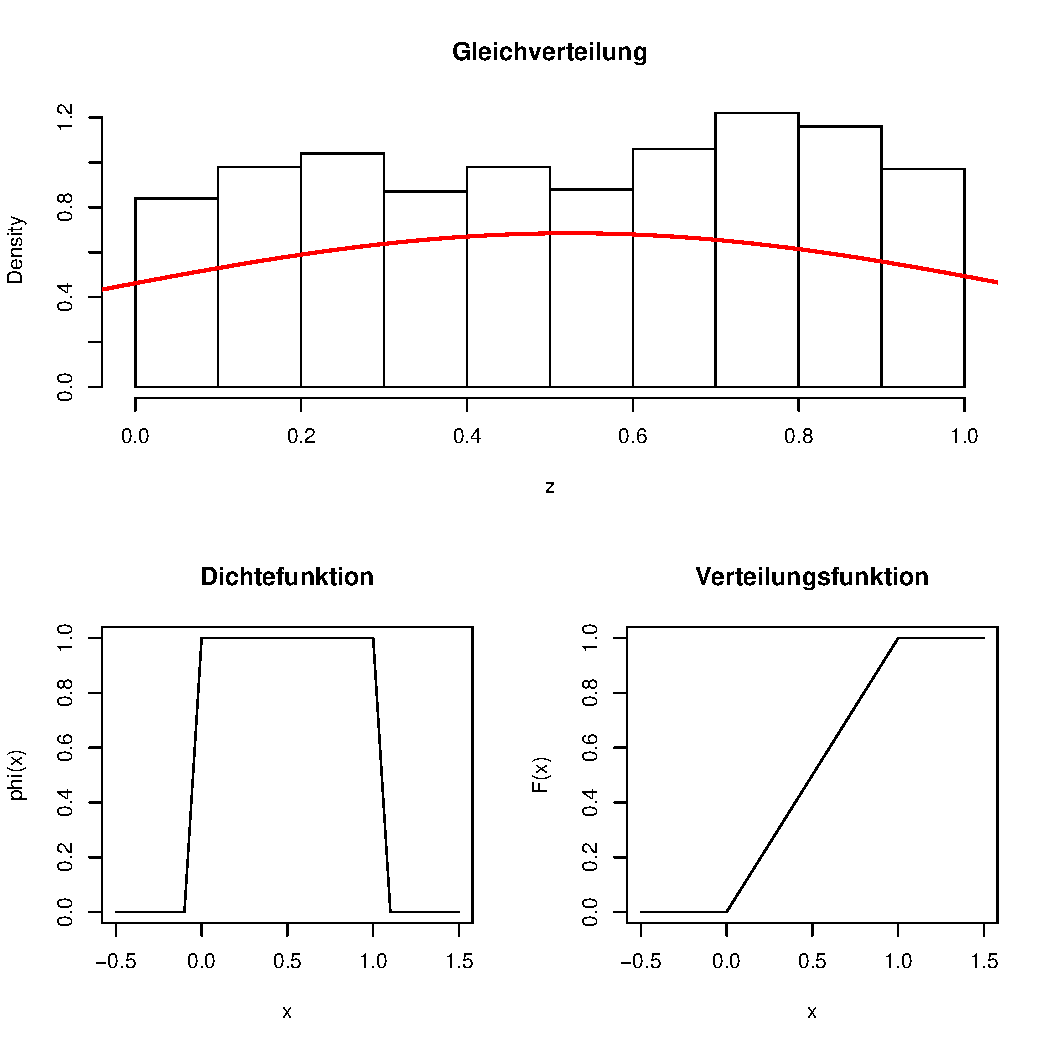
\includegraphics[width=10cm]{images/gleichverteilung.pdf}
\end{figure}

\subsubsection{Exponentialverteilung}
\begin{description}
  \item[Anwendung] Prozess ohne Erinnerungsvermögen, radioaktiver
  Zerfall, ermüdungsfreie Bauteile
  \item[Dichtefunktion] \[\varphi(x) = \begin{cases}0 & x < 0 \\ ae^{-ax} &
    x \geq 0\end{cases}\]
  \item[Verteilungsfuntkion] \[F(x) = \begin{cases}0 & x < 0 \\
    1-e^{-ax} & x \geq 0\end{cases}\]
  \item[Erwartungswert] \[E(X) = \mu = \frac{1}{a}\]
  \item[Varianz] \[\operatorname{var}(X) = \sigma^2 = \frac{1}{a^2}\]
  \item[Median] \[\operatorname{med}(X) = \frac{1}{a}\log 2\]
  \item[Wahrscheinlichkeit grosser Abweichung] Für eine
    exponentialverteilte Zufallsvariable mit dem Erwartungswert
    $\frac{1}{a}$ ist die Wahrscheinlichkeit einer Abweichung
    $\varepsilon$ vom Erwartungswert \[P(|X-\frac{1}{a}| > \varepsilon) =
    \begin{cases}e^{-a\varepsilon-1} & \varepsilon > \frac{1}{a} \\
    1 - e^{a\varepsilon-1} + e^{-a\varepsilon-1} & \varepsilon \leq
    \frac{1}{a}\end{cases}\]
  \item[MTBF] Mean Time Between Failure:
    $= \mu = \sigma = \sqrt{\operatorname{var}}$
\end{description}
\begin{figure}[!htbp]
  \centering
  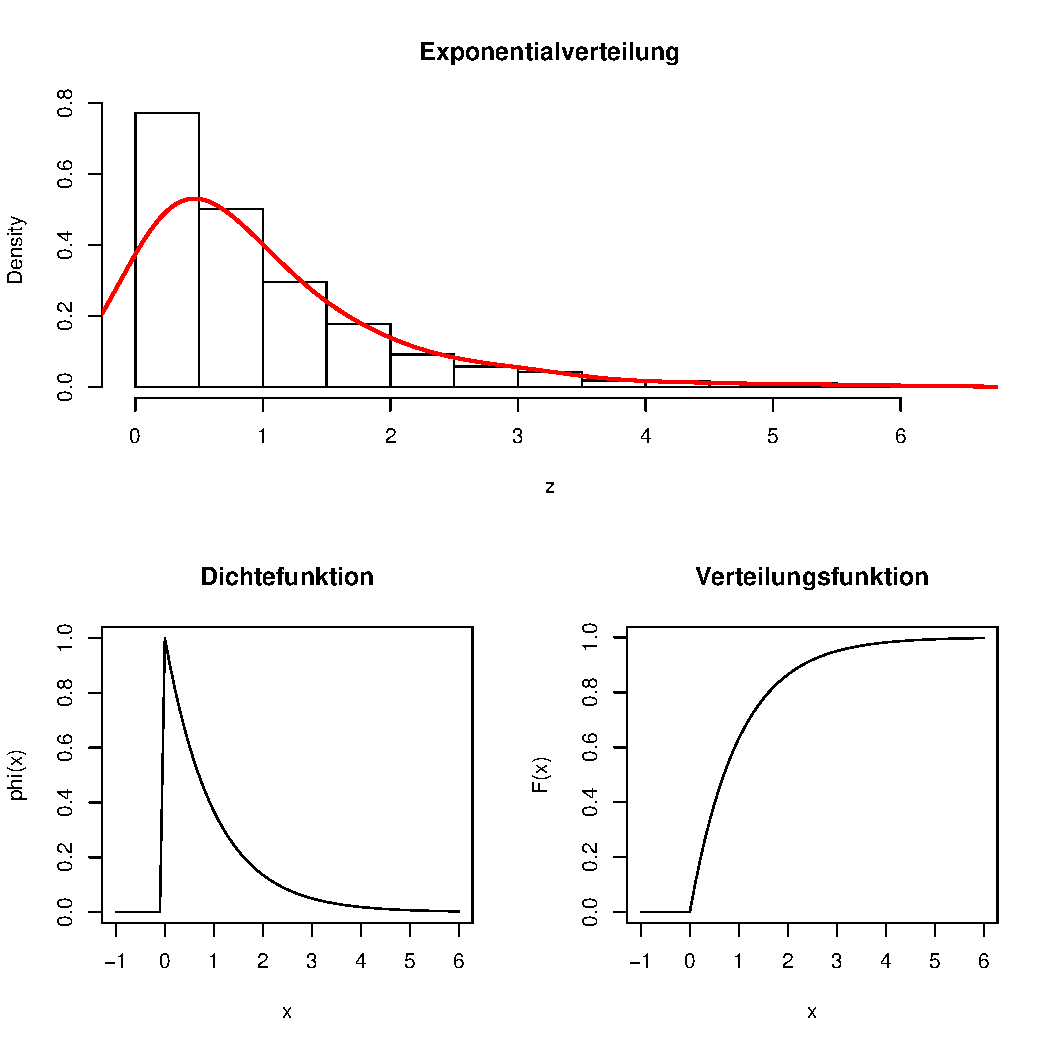
\includegraphics[width=10cm]{images/exponentialverteilung.pdf}
\end{figure}

\subsubsection{Normalverteilung / Gaussverteilung}
\begin{description}
  \item[Anwendung] Messfehler, Summe von vielen voneinander
    unabhängigenn Zufallsvariabeln, Approximation der
    Binomialverteilung, Rauschen
  \item[Dichtefunktion] \[\varphi(x) = \frac{1}{\sigma \sqrt{2\pi}} \cdot 
    e^{-\frac{1}{2}{\left(\frac{x-\mu}{\sigma}\right)}^2} =
    \frac{1}{\sigma \sqrt{2\pi}} \cdot e^{-\frac{(x-\mu)^2}{2\sigma^2}}\]
  \item[Erwartungswert] \[E(X) = \mu\]
  \item[Varianz] \[\operatorname{var}(X) = \sigma^2\]
  \item[Median] \[\operatorname{med}(X) = \mu\]
  \item[Wahrscheinlichkeit] Keine einfache Formel für
    $P(|X - E(X)| > \varepsilon)$
\end{description}
\begin{figure}[!htbp]
  \centering
  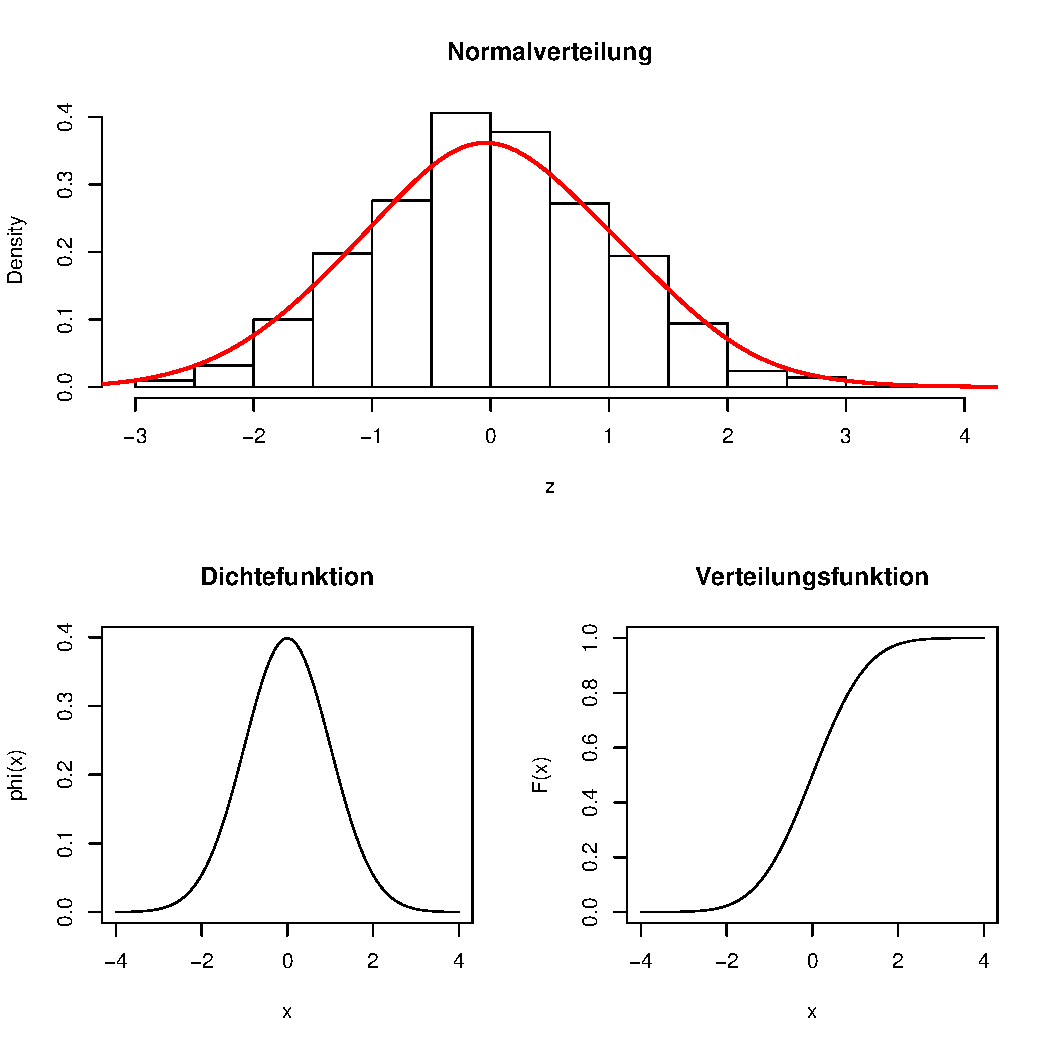
\includegraphics[width=10cm]{images/normalverteilung.pdf}
\end{figure}

% \subsection{2-Verteilung}

\subsubsection{Potenzverteilung / Pareto-Verteilung}
\begin{description}
  \item[Anwendung] Häufkeitsverteilung für skaleninvariante Prozesse,
    Einkommensverteilung Grösse und Häufigkeit von Mondkratern,
    Verkaufszahlen von Büchern, Einwohnerzahlen von Städten
  \item[Dichtefunktion] \[ \varphi(X) = \begin{cases} Cx^{-\alpha} & x \geq
    x_{min} \\ 0 & x < x_{min}\end{cases} \] Typische Werte für $\alpha$:
    $1 \leq \alpha \leq 3$
  \item[Verteilungsfunktion]
  \item[Varianz]
  \item[Median]
  \item[Wahrscheinlichkeit]
\end{description}

\subsection{Diskrete Wahrscheinlichkeitsverteilungen}
\subsubsection{Gleichverteilung}
\begin{description}
  % TODO Andere Werte
  \item[Erwartungswert] \[ E(X) = \frac{n+1}{2} \]
  \item[Varianz] \[ \operatorname{var}(X) = \frac{n^2-1}{12}\]
\end{description}

\subsubsection{Binomialverteilung}
\begin{description}
  \item[Anwendungen] Anzahl Einheiten eines Bernoulli-Ereignisses bei
    $n$ Wiederholungen ($2$ mögliche Versuchsausgänge).
  \item[Wahrscheinlichkeit] Eine Zufallsvariable mit diskreten Werten
    $k \in \{0, \dots, n\}$ heisst binomialverteilt zum Parameter $p$,
    (Wahrscheinlichkeit) wenn folgendes die Wahrscheinlichkeit des
    Wertes $k$ ist. Wahrscheinlichkeit, dass $X = 1$ k-mal eingetreten
    ist:
    \[P(X = k) = \binom{n}{k} p^k(1-p)^{n-k}\]
  \item[Verteilungsfunktion] \[F(k) = \sum_{i=0}^k \binom{n}{i} p^i(1-p)^{n-i}\]
  \item[Erwartungswert] \[E(X) = np\]
  \item[Varianz] \[\operatorname{var}(X) = np(1-p)\]
    Maximale Varianz wird erreicht bei $p = \frac{1}{2}$
  \item[Schlecht berechenbar] Ist $n$ und $p$ gross, dauert das
  berechnen der Wahrscheinlichkeit sehr lange. Dann kann man davon
  ausgehen, dass die Zufallsvariable $X$ annähernd normalverteilt ist.
\end{description}

%\subsubsection{Hypergeometrische Verteilung}

\subsubsection{Poissonverteilung}
\begin{description}
  \item[Anwendung] Anzahl Ereignisse in einem Zeitintervall, wenn die
    Zeitabstände exponentiell verteilt sind. Approximation der
    Binomialverteilung für seltene Ereignisse, die mit Rate $\lambda$
    eintreten.
  \item[Verteilungsfunktion] Sind $(X_i)1 \leq i \leq k$
    exponentialverteilte, unabhängige Zufallsvariablen, dann gilt für die
    Summe:
  \[F_{X_i+\dots+x_k}(x) = \begin{cases}1 - e^{-ax} \sum_{i=0}^{k-1}
  \frac{(ax)^i}{i!} & x \geq 0 \\ 0 & x < 0\end{cases}\]
  \item[Wahrscheinlichkeitsdichte]
  \[\varphi_{X_i+\dots+x_k}(x) = \begin{cases}a^k \frac{k^{k-1}}{(k-1)!}
  e^{-ax} & x \geq 0 \\ 0 & x < 0\end{cases}\]
  \item[Wahrscheinlichkeit] Beschreibt für $\lambda = ax$ die
    Wahrscheinlichkeit, dass in einem Zeitintervall $[0, x]$ genau $k$
    Ereignisse eintreten, wenn die Zeit zwischen den Ereignissen
    exponentialverteilt ist mit der Dichte $ae^{-ax}$ ($\lambda$ = Rate,
    in der Ereignisse auftreten).
    \[P_\lambda(k) = e^{-\lambda} \cdot \frac{\lambda^k}{k!}\]
  \item[Erwartungswert] \[E(X) = \lambda\]
  \item[Varianz] \[\operatorname{var}(X) = \lambda\]
\end{description}

\subsubsection{Poissonverteilung als Approximation für die
Binomialverteilung}
\begin{itemize}
  \item Zufallsvariable $X$ ist binomialverteilt
  \item Ist $n$ bei der Binomialverteilung gross, ist diese nicht
    durchführbar (zulange Rechenzeit).
  \item Ist $X$ annähernd normalverteilt, gilt:
    $E(X) = \mu = np$ und $\operatorname{var}(X) = \sigma^2 = np(1-p)$
\end{itemize}
Verteilfunktion:
\[ P(X \le x) = P\left(\frac{X - \mu}{\sigma} \le
  \frac{x-\mu}{\sigma}\right) = F\left(\frac{x-np}{\sqrt{np(1-p)}}\right)\]
Poissonverteilung zum Parameter $\lambda$:
\[ P_{\lambda}(k) = e^{-\lambda} \frac{\lambda^k}{k!}\]

%%%%%%%%%%%%%%%%%%%%%%%%%%%%%%%%%%%%%%%%%%%%%%%%%%%%%%%%%%%%%%%%%%%%%%%%
\section{Schätzen}
\subsection{Begriffe}
\begin{description}
  \item[Schätzer] Formel $\hat{\vartheta}(x_1, x_2, \dots, x_n)$ für
  einen Parameter wie $\mu, \sigma^2, n, p, \lambda$.
  \item Stichprobe der Zufallsvariabeln $X$, wenn die Zufallsvariabeln
    $X_i$ unabhängig und identisch zu $X$ verteilt sind.
\end{description}
\subsection{Qualitätskriterien für Schätzer}
\begin{description}
  \item[Konsistente Schätzer] Unendliche Stichproben ergeben den exakten
  Parameterwert (fast immer erfüllt).
    \[ \lim_{n \rightarrow \infty} \vartheta(X_1, \dots, X_n) \]
  \item[Erwartungstreue Schätzer] Im Mittel richtig, auch bei kleinen n.
    \[ E(\hat{\vartheta}(x_1, \dots, x_n)) = \vartheta \]
\end{description}
\subsection{Schätzer finden}
Likelihood-Funktion
\[ L(x_1, \dots, x_n) = \varphi(x_1) \cdot \ldots \cdot \varphi(x_n)\]

\subsection{Bekannte Schätzer}
\begin{description}
  \item[Stichprobenmittelwert] Der Schätzer für den
    Stichprobenmittelwert der Stichproben $X_1, \dots, X_n$ heisst:
    \[ \hat{X} = \hat{\mu}(X_1, \dots, X_n) = \frac{X_1 + \ldots +
    X_n}{n} = \frac{1}{n} \sum_{i=1}^{n} X_i \]
  \item[Stichprobenvarianz] Der Schätzer für die Stichprobenvarianz der
    Stichproben $X_1, \dots, X_n$ heisst:
    \[ S^2 = \hat{\sigma^2}(x_1, \dots, x_n) = \frac{1}{n-1}
    \sum_{i=1}^{n}(X_i - \overline{X})^2 = \frac{n}{n-1}\left( \frac{1}{n}
    \sum {x_i}^2 - \left(\frac{1}{n} \sum x_i\right)^2\right)\]
  \item[Länge eines Intervalls] Ist $X_i$ eine Stichprobe einer auf dem
    Intervall $[0, \vartheta]$ gleichverteilten Zufallsvariable $X$, dann ist
    folgende Formel ein erwartungstreuer Schätzer für die Intervallänge
    $\vartheta$:
    \[ \hat{\vartheta} = \frac{n+1}{n} \operatorname{max}(X_1, \dots, X_n)\]
  \item[Parameter $\lambda$ einer Poissonverteilung] Der Schätzer für
    den Parameter $\lambda$ einer Poissonverteilung ist:
    \[ \lambda(X_1, \dots, X_n) = \frac{1}{n} \sum_{i=1}^{n} X_i \]
  \item[Parameter $p$ einer Binomialverteilung] Der Schätzer für den
    Parameter $p$ einer Binomialkoeffizient mit den bekannten Parametern
    $m$ ist:
    \[ p(X_1, \dots, X_n) = \frac{1}{nm} \sum_{i=1}^{n} X_i \]
\end{description}

%%%%%%%%%%%%%%%%%%%%%%%%%%%%%%%%%%%%%%%%%%%%%%%%%%%%%%%%%%%%%%%%%%%%%%%%
\section{Hypothesentests - Wie wissen wir, das etwas wahr ist?}
\subsection{Aussagen}
\begin{itemize}
  \item Aussagen müssen falsifizierbar sein
  \item Positive Aussagen brauchen einen Beweis
  \item Negative Aussagen können nicht bewiesen werden
  \item Ausgangsposition ist ''wir akzeptieren nichts``
  \item Aussagen werden provisorisch akzeptier
\end{itemize}

\subsection{Begriffe}
\begin{itemize}
  \item Nullhypothese: Ausgangsposition
    (z.~B. ''Gleichviele orange wie rote Bonbons``)
  \item Hypothese: Positive falsifizierbare Aussage
    (z.~B. ``Mehr orange als rote Bonbons``)
  \begin{itemize}
    \item Falsifizierbar: Messgrösse, die entweder wahr oder falsch ist
  \end{itemize}
\end{itemize}

\subsection{Testen der Wahrscheinlichkeit eines Ereignisses (Diskret)}
\subsubsection{$\chi^2$-Test}
\begin{itemize}
  \item Nullhypothese: Farbe der Sugus ist Gleichverteilt.
  \item Hypothese: Dem ist nicht so.
\end{itemize}
Diskrepanz $D$ (Abweichung von der Nullhypothese) berechnen:
\[ D = \sum \frac{(n_i - np_i)^2}{np_i} \]

Mit Hilfe dieser Tabelle:

\begin{tabular}{|l|l|l|l|l|l|}
  \hline
  Mögliche Werte & Wahrscheinlichkeit ($p_i$) & Anzahl Ereignisse ($n_i$) & $np_i$ & $n_i - np_i$ & $\frac{(n_i - np_i)^2}{np_i}$ \\
  \hline
  \hline
  Gelb    &   0.25    &  11       &   15.75    &  4.75    &  1.432 \\
  Orange  &   0.25    &  23       &   15.75    &  7.25    &  3.34  \\
  Rot     &   0.25    &  10       &   15.75    &  5.75    &  2.09  \\
  Grün    &   0.25    &  19       &   15.75    &  3.25    &  0.67  \\
  \hline
  \hline
  Total   &   1       &  63 = $n$ &   15.75    &          & $D$    \\
  \hline
\end{tabular}


Die Diskrepanz $D$ ist für genügend grosse $n$ annhährend $\chi^2$
verteilt mit $k$ Freiheitsgraden ($k = $ Anzahl Ausgänge $-1$).

Ist $D < D_{\text{Krit}}$, gibt es keinen Grund an der Nullhypothese zu
zweifeln.

Einschränkungen:
\begin{itemize}
  \item Bei wenigen Testdaten nicht anwendbar
  \item Ist $p_i$ klein, sind sehr viele Beobachtungen nötig
  \item Faustregel: Jedes Intervall sollte mindestens 5 Einträge haben:
    $n_i \geq 5$
\end{itemize}

\subsection{Testen der Wahrscheinlichkeit eines Ereignisses (Stetig)}
\subsubsection{Kolmogoroff-Smirnov-Test}
\begin{itemize}
  \item Nullhypothese: Daten sind gemäss der Verteilungsfunktion $F$
    verteilt.
  \item Hypothese: ``Das ist nicht so.''
  \item Idee: Unterschied zwischen der Verteilfunktion $F$
    und der gemessenen Verteilfunktion $F_{\text{Empirisch}}$ messen.
  \item Gesucht: Grösste Abweichung zwischen $F$ und $F_{\text{Empirisch}}$
\end{itemize}

\[ F_{\text{Empirisch}}(x) = \frac{|\{x_i | X_i \leq x\}|}{n} \]

Berechnung mit Tabelle (Die $x_j$ Werte müssen aufsteigend sortiert
sein!):

\begin{tabular}{|l|l|l|l|l|}
  \hline
  $j$        & $x_j$     & $F(x_j)$    & $\frac{j}{n}-F(x_i)$  & $F(x_j) - \frac{j-1}{n}$ \\
  \hline
  \hline
  1         &           &           &            &          \\
  2         &           &           &            &          \\
  $\vdots$  &           &           &            &          \\
  n         &           &           &            &          \\
  \hline
  \hline
          &           &  & $\operatorname{max}(...)$ & $\operatorname{max}(...)$ \\
  \hline
\end{tabular}


\[ K_n^+ = \sqrt{n} \cdot \max_{-\infty<x<\infty} \left(\frac{j}{n} - F(x_j)\right)
, \qquad
K_n^- = \sqrt{n} \cdot \max_{-\infty<x<\infty} \left(F(x_j) - \frac{j-1}{n} \right) \]

Der kritische Wert $K_{\text{krit}}$ kann man aus der Tabelle auslesen.
Ist $k_{\text{krit}} > K^\pm$, ist die Nullhypothese falsch.

Wie ist die Verteilung von $F(X)$?

\[ F_{F(X)}(X) = P(F(X) \leq x) = P(X \leq F^{-1}(x)) = F_X(F^{-1}(x)) =
x \]

\subsubsection{t-Test}
\begin{itemize}
  \item Nullhypothese: Zwischen zwei Messreihen gibt es kein Unterschied
    (Messreihen sind normalverteilt).
  \item Hypothese: Es gibt einen Unterschied.
  \item Nützlich, wenn beide Messreihen grosse Unterschiede haben
    (Varianz ist gross)
  \item Anzahl Messungen für $X$: $n$ und Anzahl Messungen für $Y$: $m$
  \item Zwei Mittelwerte der Messreihe $X$ unx $Y$:
    $\overline{X} = \mu_x$ und $\overline{Y} = \mu_y$
  \item Varianz von $X$: ${S_X}^2 = \operatorname{var}(X)$ und Varianz
    von $Y$: $d {S_Y}^2 = \operatorname{var}(Y)$
\end{itemize}

\[ T = \frac{\overline{X} - \overline{Y}}{\sqrt{(n-1) {S_X}^2 + (m-1)
{S_Y}^2}} \cdot \sqrt{\frac{nm(n+m-2)}{n+m}}\]

$T$ ist t-Verteilt (vgl. Tabelle). Man legt ein $\alpha$ fest und berechnet den
kritischen Wert. Ist $t > t_{krit}$, verwirft man die Nullhypothese.

%%%%%%%%%%%%%%%%%%%%%%%%%%%%%%%%%%%%%%%%%%%%%%%%%%%%%%%%%%%%%%%%%%%%%%%%
\section{Filter}
\subsection{Kalman-Filter}
\begin{itemize}
  \item Anwendung: GPS-Empfänger, Mondflug, Scheitelbestimmung einer
    Raketenbahn
\end{itemize}

%%%%%%%%%%%%%%%%%%%%%%%%%%%%%%%%%%%%%%%%%%%%%%%%%%%%%%%%%%%%%%%%%%%%%%%%
\section{Anhang}
\subsection{Summenformeln}
\[ \begin{aligned}
  \sum_{i=1}^{n}i     & = \frac{n(n+1)}{2} \\
  \sum_{i=1}^{n}i^2   & = \frac{n(n+1)(2n+1)}{6} \\
  \sum_{i=1}^{n}i^3   & = \left(\frac{n(n+1)}{2}\right)^2 \\
\end{aligned} \]

\subsection{Tabellen}
Die Tabellen wurden aus dem Skript der Vorlesung von Herr Müller
übernommen.
\subsubsection{Quantilen der Normalverteilung}
\begin{figure}[!h]
  \begin{center}
    \scriptsize
    \begin{tabular}{|l|r|}
      \hline
      $p$&$x$ \\
      \hline
      0.75&0.6745 \\
      0.8&0.8416 \\
      0.9&1.2816 \\
      0.95&1.6449 \\
      0.975&1.9600 \\
      0.99&2.3263 \\
      0.995&2.5758 \\
      0.999&3.0902 \\
      0.9995&3.2905 \\
      \hline
    \end{tabular}
  \end{center}
\end{figure}
\begin{itemize}
  \item Muss Standardisiert sein: Mit $E(X) = 0$ und 
    $\operatorname{var} = 1$ 
\end{itemize}

\pagebreak
\subsubsection{Verteilungsfunktion der Normalverteilung}
\begin{figure}[!h]
\begin{center}
\scriptsize
\begin{tabular}{|r|rrrrrrrrrr|}
\hline
$x$&+0.00&+0.01&+0.02&+0.03&+0.04&+0.05&+0.06&+0.07&+0.08&+0.09\\
\hline
0.0&0.5000&0.5040&0.5080&0.5120&0.5160&0.5199&0.5239&0.5279&0.5319&0.5359\\
0.1&0.5398&0.5438&0.5478&0.5517&0.5557&0.5596&0.5636&0.5675&0.5714&0.5753\\
0.2&0.5793&0.5832&0.5871&0.5910&0.5948&0.5987&0.6026&0.6064&0.6103&0.6141\\
0.3&0.6179&0.6217&0.6255&0.6293&0.6331&0.6368&0.6406&0.6443&0.6480&0.6517\\
0.4&0.6554&0.6591&0.6628&0.6664&0.6700&0.6736&0.6772&0.6808&0.6844&0.6879\\
0.5&0.6915&0.6950&0.6985&0.7019&0.7054&0.7088&0.7123&0.7157&0.7190&0.7224\\
0.6&0.7257&0.7291&0.7324&0.7357&0.7389&0.7422&0.7454&0.7486&0.7517&0.7549\\
0.7&0.7580&0.7611&0.7642&0.7673&0.7704&0.7734&0.7764&0.7794&0.7823&0.7852\\
0.8&0.7881&0.7910&0.7939&0.7967&0.7995&0.8023&0.8051&0.8078&0.8106&0.8133\\
0.9&0.8159&0.8186&0.8212&0.8238&0.8264&0.8289&0.8315&0.8340&0.8365&0.8389\\
1.0&0.8413&0.8438&0.8461&0.8485&0.8508&0.8531&0.8554&0.8577&0.8599&0.8621\\
1.1&0.8643&0.8665&0.8686&0.8708&0.8729&0.8749&0.8770&0.8790&0.8810&0.8830\\
1.2&0.8849&0.8869&0.8888&0.8907&0.8925&0.8944&0.8962&0.8980&0.8997&0.9015\\
1.3&0.9032&0.9049&0.9066&0.9082&0.9099&0.9115&0.9131&0.9147&0.9162&0.9177\\
1.4&0.9192&0.9207&0.9222&0.9236&0.9251&0.9265&0.9279&0.9292&0.9306&0.9319\\
1.5&0.9332&0.9345&0.9357&0.9370&0.9382&0.9394&0.9406&0.9418&0.9429&0.9441\\
1.6&0.9452&0.9463&0.9474&0.9484&0.9495&0.9505&0.9515&0.9525&0.9535&0.9545\\
1.7&0.9554&0.9564&0.9573&0.9582&0.9591&0.9599&0.9608&0.9616&0.9625&0.9633\\
1.8&0.9641&0.9649&0.9656&0.9664&0.9671&0.9678&0.9686&0.9693&0.9699&0.9706\\
1.9&0.9713&0.9719&0.9726&0.9732&0.9738&0.9744&0.9750&0.9756&0.9761&0.9767\\
2.0&0.9772&0.9778&0.9783&0.9788&0.9793&0.9798&0.9803&0.9808&0.9812&0.9817\\
2.1&0.9821&0.9826&0.9830&0.9834&0.9838&0.9842&0.9846&0.9850&0.9854&0.9857\\
2.2&0.9861&0.9864&0.9868&0.9871&0.9875&0.9878&0.9881&0.9884&0.9887&0.9890\\
2.3&0.9893&0.9896&0.9898&0.9901&0.9904&0.9906&0.9909&0.9911&0.9913&0.9916\\
2.4&0.9918&0.9920&0.9922&0.9925&0.9927&0.9929&0.9931&0.9932&0.9934&0.9936\\
2.5&0.9938&0.9940&0.9941&0.9943&0.9945&0.9946&0.9948&0.9949&0.9951&0.9952\\
2.6&0.9953&0.9955&0.9956&0.9957&0.9959&0.9960&0.9961&0.9962&0.9963&0.9964\\
2.7&0.9965&0.9966&0.9967&0.9968&0.9969&0.9970&0.9971&0.9972&0.9973&0.9974\\
2.8&0.9974&0.9975&0.9976&0.9977&0.9977&0.9978&0.9979&0.9979&0.9980&0.9981\\
2.9&0.9981&0.9982&0.9982&0.9983&0.9984&0.9984&0.9985&0.9985&0.9986&0.9986\\
3.0&0.9987&0.9987&0.9987&0.9988&0.9988&0.9989&0.9989&0.9989&0.9990&0.9990\\
\hline
\end{tabular}
\end{center}
\end{figure}

\begin{itemize}
  \item In \texttt{R}: \texttt{pnorm(x)}
\end{itemize}

\pagebreak
\subsubsection{Quantilen der $\chi^2$-Verteilung}
\begin{figure}[h!]
\begin{center}
\scriptsize
\begin{tabular}{|r|rrr|rrr|rrr|}
\hline
\strut$k$&$p=0.01$&$p=0.05$&$p=0.1$&$p=0.25$&$p=0.5$&$p=0.75$&$p=0.9$&$p=0.95$&$p=0.99$\\
\hline
1&0.000&0.004&0.016&0.102&0.455&1.323&2.706&3.841&6.635\\
2&0.020&0.103&0.211&0.575&1.386&2.773&4.605&5.991&9.210\\
3&0.115&0.352&0.584&1.213&2.366&4.108&6.251&7.815&11.345\\
4&0.297&0.711&1.064&1.923&3.357&5.385&7.779&9.488&13.277\\
5&0.554&1.145&1.610&2.675&4.351&6.626&9.236&11.070&15.086\\
6&0.872&1.635&2.204&3.455&5.348&7.841&10.645&12.592&16.812\\
7&1.239&2.167&2.833&4.255&6.346&9.037&12.017&14.067&18.475\\
8&1.646&2.733&3.490&5.071&7.344&10.219&13.362&15.507&20.090\\
9&2.088&3.325&4.168&5.899&8.343&11.389&14.684&16.919&21.666\\
10&2.558&3.940&4.865&6.737&9.342&12.549&15.987&18.307&23.209\\
11&3.053&4.575&5.578&7.584&10.341&13.701&17.275&19.675&24.725\\
12&3.571&5.226&6.304&8.438&11.340&14.845&18.549&21.026&26.217\\
13&4.107&5.892&7.042&9.299&12.340&15.984&19.812&22.362&27.688\\
14&4.660&6.571&7.790&10.165&13.339&17.117&21.064&23.685&29.141\\
15&5.229&7.261&8.547&11.037&14.339&18.245&22.307&24.996&30.578\\
16&5.812&7.962&9.312&11.912&15.338&19.369&23.542&26.296&32.000\\
17&6.408&8.672&10.085&12.792&16.338&20.489&24.769&27.587&33.409\\
18&7.015&9.390&10.865&13.675&17.338&21.605&25.989&28.869&34.805\\
19&7.633&10.117&11.651&14.562&18.338&22.718&27.204&30.144&36.191\\
20&8.260&10.851&12.443&15.452&19.337&23.828&28.412&31.410&37.566\\
21&8.897&11.591&13.240&16.344&20.337&24.935&29.615&32.671&38.932\\
22&9.542&12.338&14.041&17.240&21.337&26.039&30.813&33.924&40.289\\
23&10.196&13.091&14.848&18.137&22.337&27.141&32.007&35.172&41.638\\
24&10.856&13.848&15.659&19.037&23.337&28.241&33.196&36.415&42.980\\
25&11.524&14.611&16.473&19.939&24.337&29.339&34.382&37.652&44.314\\
26&12.198&15.379&17.292&20.843&25.336&30.435&35.563&38.885&45.642\\
27&12.879&16.151&18.114&21.749&26.336&31.528&36.741&40.113&46.963\\
28&13.565&16.928&18.939&22.657&27.336&32.620&37.916&41.337&48.278\\
29&14.256&17.708&19.768&23.567&28.336&33.711&39.087&42.557&49.588\\
30&14.953&18.493&20.599&24.478&29.336&34.800&40.256&43.773&50.892\\
50&29.707&34.764&37.689&42.942&49.335&56.334&63.167&67.505&76.154\\
100&70.065&77.929&82.358&90.133&99.334&109.141&118.498&124.342&135.807\\
500&429.388&449.147&459.926&478.323&499.333&520.950&540.930&553.127&576.493\\
1000&898.912&927.594&943.133&969.484&999.333&1029.790&1057.724&1074.679&1106.969\\
\hline
\end{tabular}
\end{center}
\end{figure}

\begin{itemize}
  \item $k$ = Freiheitsgrade = Anzahl Ausgänge - 1
  \item $p = 1 - \alpha$
  \item Wenn nichts anderes angegeben: $p = 0.95$ wählen.
\end{itemize}

\pagebreak
\subsubsection{Quantilen für den Kolmogorov-Smirnov-Test}
\begin{figure}[h!]
\scriptsize
\begin{center}
\begin{tabular}{|r|rrr|rrr|rrr|}
\hline
$n$&$p=0.01$&$p=0.05$&$p=0.1$&$p=0.25$&$p=0.5$&$p=0.75$&$p=0.9$&$p=0.95$&$p=0.99$\\
\hline
1&0.01000&0.05000&0.10000&0.25000&0.50000&0.75000&0.90000&0.95000&0.99000\\
2&0.01400&0.06749&0.12955&0.29289&0.51764&0.70711&0.96700&1.09799&1.27279\\
3&0.01699&0.07919&0.14714&0.31117&0.51469&0.75394&0.97828&1.10166&1.35889\\
4&0.01943&0.08789&0.15899&0.32023&0.51104&0.76419&0.98531&1.13043&1.37774\\
5&0.02152&0.09471&0.16750&0.32490&0.52449&0.76741&0.99948&1.13916&1.40242\\
6&0.02336&0.10022&0.17385&0.32717&0.53193&0.77028&1.00520&1.14634&1.41435\\
7&0.02501&0.10479&0.17873&0.32804&0.53635&0.77552&1.00929&1.15373&1.42457\\
8&0.02650&0.10863&0.18256&0.32802&0.53916&0.77971&1.01346&1.15859&1.43272\\
9&0.02786&0.11191&0.18560&0.32745&0.54109&0.78246&1.01731&1.16239&1.43878\\
10&0.02912&0.11473&0.18803&0.32975&0.54258&0.78454&1.02016&1.16582&1.44397\\
11&0.03028&0.11718&0.19000&0.33304&0.54390&0.78633&1.02249&1.16885&1.44837\\
12&0.03137&0.11933&0.19160&0.33570&0.54527&0.78802&1.02458&1.17139&1.45207\\
13&0.03239&0.12123&0.19291&0.33789&0.54682&0.78966&1.02649&1.17357&1.45527\\
14&0.03334&0.12290&0.19396&0.33970&0.54856&0.79122&1.02823&1.17552&1.45810\\
15&0.03424&0.12439&0.19482&0.34122&0.55002&0.79259&1.02977&1.17728&1.46060\\
16&0.03509&0.12573&0.19552&0.34250&0.55123&0.79377&1.03113&1.17888&1.46283\\
17&0.03589&0.12692&0.19607&0.34360&0.55228&0.79482&1.03237&1.18032&1.46483\\
18&0.03665&0.12799&0.19650&0.34454&0.55319&0.79578&1.03351&1.18162&1.46664\\
19&0.03738&0.12895&0.19684&0.34535&0.55400&0.79667&1.03457&1.18282&1.46830\\
20&0.03807&0.12982&0.19709&0.34607&0.55475&0.79752&1.03555&1.18392&1.46981\\
30&0.04354&0.13510&0.20063&0.35087&0.56047&0.80362&1.04243&1.19164&1.48009\\
50&0.05005&0.13755&0.20794&0.35713&0.56644&0.80988&1.04933&1.19921&1.48969\\
100&0.05698&0.14472&0.21370&0.36331&0.57269&0.81634&1.05627&1.20666&1.49864\\
200&0.06049&0.14887&0.21816&0.36784&0.57725&0.82099&1.06117&1.21180&1.50458\\
\hline
\end{tabular}
\end{center}
\end{figure}

\begin{itemize}
  \item Werte entsprechen $k_{\text{Krint}}$
  \item $p = 1 - \alpha$
\end{itemize}

\pagebreak
\subsubsection{Quantilen der t-Verteilung}
\begin{figure}[h!]
\scriptsize
\begin{center}
\begin{tabular}{|r|rrrrrrr|}
\hline
$k$&0.75&0.8&0.9&0.95&0.975&0.99&0.995\\
\hline
1&1.0000&1.3764&3.0777&6.3138&12.7062&31.8205&63.6567\\
2&0.8165&1.0607&1.8856&2.9200&4.3027&6.9646&9.9248\\
3&0.7649&0.9785&1.6377&2.3534&3.1824&4.5407&5.8409\\
4&0.7407&0.9410&1.5332&2.1318&2.7764&3.7469&4.6041\\
5&0.7267&0.9195&1.4759&2.0150&2.5706&3.3649&4.0321\\
6&0.7176&0.9057&1.4398&1.9432&2.4469&3.1427&3.7074\\
7&0.7111&0.8960&1.4149&1.8946&2.3646&2.9980&3.4995\\
8&0.7064&0.8889&1.3968&1.8595&2.3060&2.8965&3.3554\\
9&0.7027&0.8834&1.3830&1.8331&2.2622&2.8214&3.2498\\
10&0.6998&0.8791&1.3722&1.8125&2.2281&2.7638&3.1693\\
11&0.6974&0.8755&1.3634&1.7959&2.2010&2.7181&3.1058\\
12&0.6955&0.8726&1.3562&1.7823&2.1788&2.6810&3.0545\\
13&0.6938&0.8702&1.3502&1.7709&2.1604&2.6503&3.0123\\
14&0.6924&0.8681&1.3450&1.7613&2.1448&2.6245&2.9768\\
15&0.6912&0.8662&1.3406&1.7531&2.1314&2.6025&2.9467\\
16&0.6901&0.8647&1.3368&1.7459&2.1199&2.5835&2.9208\\
17&0.6892&0.8633&1.3334&1.7396&2.1098&2.5669&2.8982\\
18&0.6884&0.8620&1.3304&1.7341&2.1009&2.5524&2.8784\\
19&0.6876&0.8610&1.3277&1.7291&2.0930&2.5395&2.8609\\
20&0.6870&0.8600&1.3253&1.7247&2.0860&2.5280&2.8453\\
21&0.6864&0.8591&1.3232&1.7207&2.0796&2.5176&2.8314\\
22&0.6858&0.8583&1.3212&1.7171&2.0739&2.5083&2.8188\\
23&0.6853&0.8575&1.3195&1.7139&2.0687&2.4999&2.8073\\
24&0.6848&0.8569&1.3178&1.7109&2.0639&2.4922&2.7969\\
25&0.6844&0.8562&1.3163&1.7081&2.0595&2.4851&2.7874\\
26&0.6840&0.8557&1.3150&1.7056&2.0555&2.4786&2.7787\\
27&0.6837&0.8551&1.3137&1.7033&2.0518&2.4727&2.7707\\
28&0.6834&0.8546&1.3125&1.7011&2.0484&2.4671&2.7633\\
29&0.6830&0.8542&1.3114&1.6991&2.0452&2.4620&2.7564\\
30&0.6828&0.8538&1.3104&1.6973&2.0423&2.4573&2.7500\\
50&0.6794&0.8489&1.2987&1.6759&2.0086&2.4033&2.6778\\
100&0.6770&0.8452&1.2901&1.6602&1.9840&2.3642&2.6259\\
500&0.6750&0.8423&1.2832&1.6479&1.9647&2.3338&2.5857\\
$10^3$&0.6747&0.8420&1.2824&1.6464&1.9623&2.3301&2.5808\\
$10^4$&0.6745&0.8417&1.2816&1.6450&1.9602&2.3267&2.5763\\
$10^5$&0.6745&0.8416&1.2816&1.6449&1.9600&2.3264&2.5759\\
$10^6$&0.6745&0.8416&1.2816&1.6449&1.9600&2.3264&2.5758\\
\hline
\end{tabular}
\end{center}
\end{figure}

\begin{itemize}
  \item Freiheitsgrade: $k = n + m - 2$
\end{itemize}

